% Class

\documentclass[12pt]{article}


% Info

\title{Babble: Learning Grammar Structure with Generative Adversarial Networks\thanks{\url{https://github.com/bclarkx2/babble}}}
\author{Brian Clark, CWRU}

\date{\today}

% Packages

% \usepackage{amsmath}
% \usepackage{nccmath}
% \usepackage{enumerate}
% \usepackage{bm}
% \usepackage{textcomp}
% \usepackage{numproof}
% \usepackage{math_shortcuts}
\usepackage{listings}
\usepackage{float}
\usepackage{blindtext}
\usepackage{graphicx}
\usepackage{cite}
\usepackage{doi}
\usepackage{siunitx}
\usepackage{hyperref}

% Settings

\setlength{\parindent}{0pt}
\setlength{\parskip}{1em}
\graphicspath{ {img/} }


% Commands


% Document

\begin{document}
\maketitle
\tableofcontents

\abstract{This is the text of the abstract}

\section{Introduction}

\subsection{Problem}

The English language is undeniably a complex construct. English grammar is composed of dozens of rules, many of which are only loosely applied. The vocabulary is incredibly vast, and growing everyday. English is consistently rated one of the most difficult world languages for new speakers to learn.

And yet, even young children are capable of producing speech that is widely accepted as "English" -- at least, most of the time. Clearly, the human brain has a well developed capability for internalizing the deep structure of a language like English and generating examples that match that structure.

This naturally leads to the question: can intelligences other than human brains perform a similar feat? The purpose of this project is to produce a deep learning network that, given examples of text from a language, is able to produce text samples that comply with the rules of that language.

\subsection{Grammar}

The first challenge built into this learning problem is the definition of a language.

A approach to language definition is to think of a language as a set of formal rules called a grammar\cite{nltk_book}. Any piece of text satisfying the rules of the grammar can be considered part of the language inquestion. This grammar can be thought of as an operational definition of a language.

This leads to a natural conclusion in the realm of generative networks: a grammar could serve as a loss function for a network. The network would be rewarded for creating a grammatical sentence and penalized for created a non-grammatical sentence.

The limitations with this approach are the same as the limitations for grammars in general. For any sufficiently complex language, it becomes difficult to write a correct and complete grammar describing the language. For example, there is no one extant grammar that is widely regarded to represent the entirety of the English language. It may not even be possible to create such a grammar.

Without the feedback provided by a formal grammar, there is still one source of grammaticality available to us: actual sentences. Ideally, the generative network could use an existing corpus of sentences in a language as the basis for building a model of the language. Using data itself to glean structure rather than a set of predesigned rules is a mainstay of machine learning. This is the approach followed in this project.

\subsection{Generative Adversarial Networks}

A tool explored in this project is a deep learning model known as Generative Adversarial Networks \cite{gen_adv_model}.

The idea behind the generative adversarial approach is to split the network into two subnetworks, each with a distinct role:

\begin{itemize}
    \item \textbf{Discriminator}: The discriminator is trained to recognize the difference between examples that meet certain criteria and examples that do not. For example, the discriminator would be able to tell if a given sentence was grammatical or not in a language.
    \item \textbf{Generator}: This subnetwork is responsible for transforming random noise inputs into samples that meet the criteria being judged for by the discriminator. In this example, the generator would attempt to create phrases out of random noise that follow the rules of a language.
\end{itemize}

The insight behind this model, however, is the interplay between the two subsystem. The outputs from the generator are fed into the discriminator and labelled as negative examples. This creates a feedback loop where the discriminator gets ever better at distinguishing fake sentences from real sentences which pushes the generator to produce more realistic sentences.

\section{Background}
    ???

\section{Approach}

To accomplish the task of generating realistic text, I took the following steps.

\begin{enumerate}
    \item Established network model
    \item Created grammar representation
    \item Developed network implementations
    \item Devised several learning 'modes'
    \item Tuned specific network hyperparameters
\end{enumerate}

The following sections describe each of these steps.

\subsection{Network Model}

\begin{figure}[ht]
    \centering
    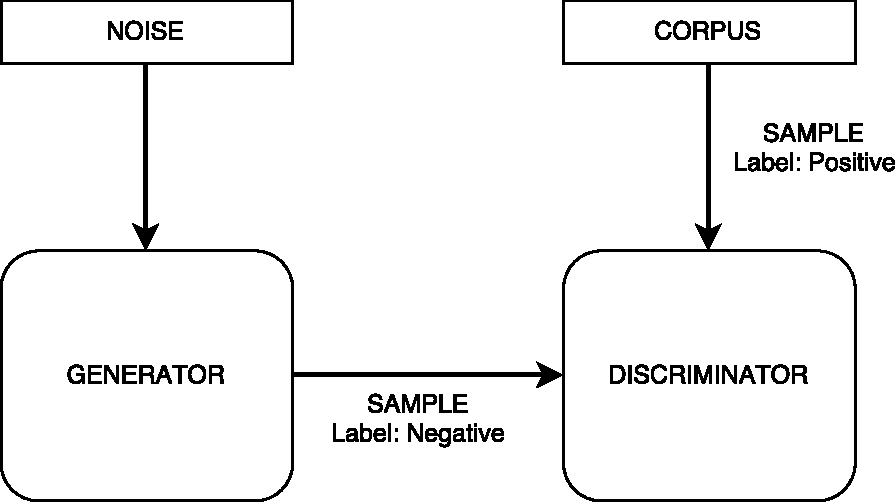
\includegraphics[scale=0.5]{img/network_model.pdf}
    \caption{Network Model}
    \label{fig:net_model}
\end{figure}

The generator takes as input a vector of random noise data, generated using the \texttt{numpy.random} module. It produces a vector of index values, where each index maps to a given word from the language's dictionary. In essence, therefore, the ouput from the generator is a sentence, as each word index in the output vector can be mapped to a word and the list of words forms a sentence.

The discriminator's input, on the other hand, is a vector of word indices. These can be drawn either from the corpus of actual sentences or from the generator itself. The discriminator is then responsible for generating a boolean classification value representing whether or not the given sentence is grammatical.

\subsection{Grammar}

As mentioned above, we cannot necessarily write a grammar that encapsulates all the complexity of the entire English language. However, it is straightforward to create a context-free grammar that succinctly describes a subset of all possible English sentences.

\subsubsection{Interface}

As an intermediate step to training a network to produce English sentences, this project provides an interface for defining smaller grammars and generating sentences that use them.

Figure \ref{fig:grammar} shows the interface developed for this purpose.
\begin{figure}[ht]
    \centering
    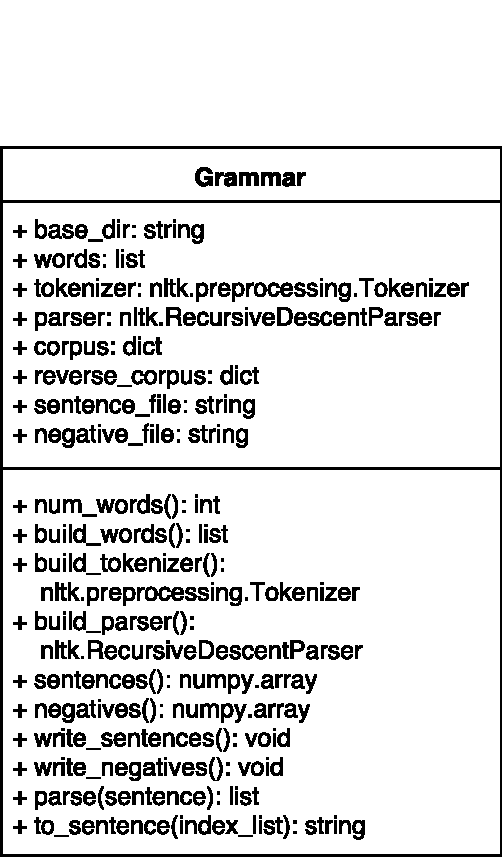
\includegraphics[trim={0 0 0 2.45cm},scale=0.7,clip]{img/grammar.pdf}
    \caption{Grammar interface}
    \label{fig:grammar}
\end{figure}

\subsubsection{Tools}

To actually represent the rules of this grammar, the \texttt{nltk} (Natural Language Toolkit) Python package provides several useful tools \cite{nltk_book}. Namely, they provide a format for describing the rules of a grammar (as detailed in the next section) and several algorithms for parsing said grammars. This project makes use of the recursive descent parser.

\subsubsection{Implementations}

Using the interface described above, this project implements the following grammars:\\

\textbf{SimpleGrammar}

This grammar represents a very small subset of English language sentences. In this language, all sentences take the form ``subject verb object'', and the total vocabulary is just 20 words. Please see Figure \ref{fig:simple_grammar} for a formal description of this context-free grammar.

\begin{figure}[ht]
    \centering
    \begin{lstlisting}
        S -> N V O
        N -> 'John'
        N -> 'Mary'
        N -> 'Alex'
        N -> 'Jack'
        N -> 'Nate'
        N -> 'Wallace'
        N -> 'Kumail'
        N -> 'Mahmoud'
        N -> 'Pierre'
        N -> 'Katrina'
        V -> 'saw'
        V -> 'found'
        V -> 'threw'
        V -> 'lost'
        O -> 'pie'
        O -> 'cheese'
        O -> 'milk'
        O -> 'grapes'
        O -> 'apples'
        O -> 'pears'
    \end{lstlisting}
    \caption{SimpleGrammar representation}
    \label{fig:simple_grammar}
\end{figure}

\subsection{Network Implementation}

The deep learning networks in Babble are implemented using the \texttt{keras} Python library, and designed to run with TensorFlow as the backend tensor manipulation framework \cite{chollet2015keras} \cite{tensorflow}.

The following sections describe some of the specific network implementations used, and the reasoning behind them. \\

\subsubsection{Generators}

Source code for the generators may be found in \texttt{generator.py}

\noindent \textbf{dense\_only\_gen} \\

This generator is composed of only dense layers. It follows the network layout described in Figure \ref{fig:dense_only_gen}.

The reasoning behind this network is to provide a basic generator model with no extra frills. Throw a bunch of neurons at the problem, and see what fits.

\begin{figure}[ht]
    \centering
    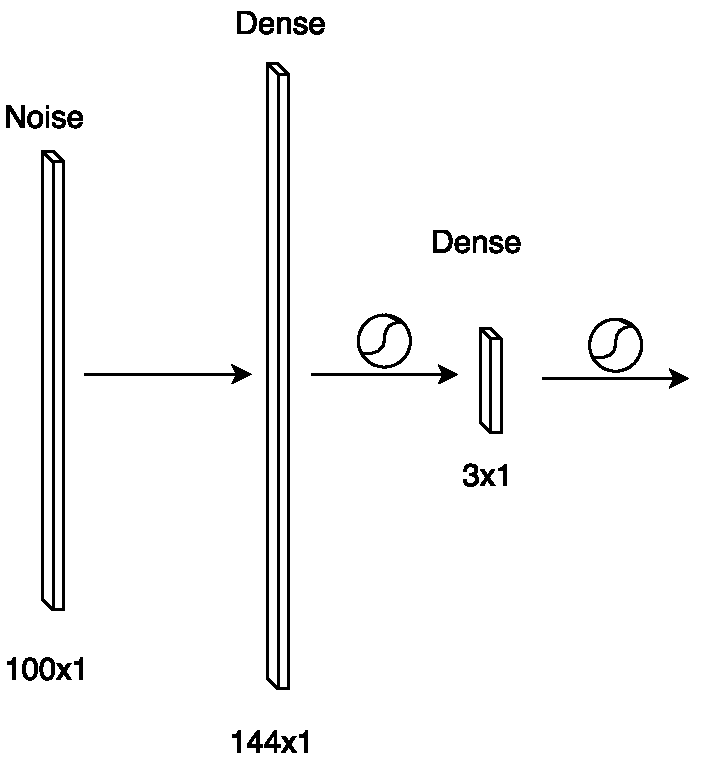
\includegraphics[scale=0.65]{img/dense_only_gen}
    \caption{dense\_only\_gen network layout}
    \label{fig:dense_only_gen}
\end{figure}

\subsubsection{Discriminators}

Source code for the discriminators can be found in \texttt{babble/discriminator.py}

\noindent \textbf{no\_conv\_disc} \\

The following discriminator is implemented without any convolution layers using the network layout described in Figure \ref{fig:no_conv_disc}

\begin{figure}[ht]
    \centering
    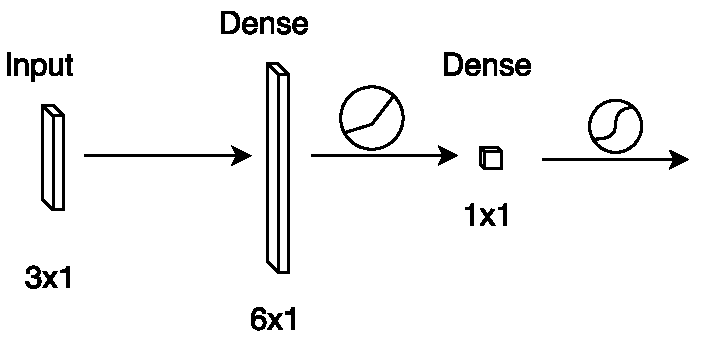
\includegraphics{no_conv_disc.pdf}
    \caption{no\_conv\_disc network layout}
    \label{fig:no_conv_disc}
\end{figure}

\subsection{Learning Modes}

With the basic network structure defined, the next step is to exercise the learning system in different ways to see interesting results. Here are the three different modes employed:

\subsubsection{Grammaticality Training}

In this mode, only the discriminator is trained. Here are the steps involved:
\begin{enumerate}
    \item A Grammar object (Figure \ref{fig:grammar}) is generated
    \item That Grammar object is used to generate many examples of valid sentences and many examples of invalid sentences.
    \item The discriminator is trained on these examples.
    \begin{itemize}
        \item Using \texttt{keras.layers.Sequential.fit}
        \item RMSProp optimization
        \item Binary cross entropy loss function
        \begin{itemize}
            \item Learning rate: \num{2e-3}
            \item Decay: \num{6e-8}
        \end{itemize}
        \item Batches of size 32
        \item Validation split: 10\%
    \end{itemize}
\end{enumerate}

\subsubsection{Oracle Training}

This learning mode is designed to train the generator alone.

Steps:
\begin{enumerate}
    \item Train the discriminator using the Grammaticality Training mode described above.
    \item Fix the weights in the discriminator.
    \item Feed the combined model (\ref{fig:net_model}) with random noise and label it positive (i.e. that it corresponds to a valid sentence). The trained discriminator will penalize the generator if it doesn't produce a valid sentence.
    \begin{itemize}
        \item Binary cross entropy loss function
        \begin{itemize}
            \item Learning rate: \num{1e-3}
            \item Decay: \num{0.0}
        \end{itemize}
        \item Batches of size 1000
    \end{itemize}
    \item Repeat until the loss is reliably low
\end{enumerate}

\subsubsection{Adversarial Training}

The adversarial training mode is the main training mode for this project.

\begin{enumerate}
    \item Select some valid sentences from the corpus. Label them as positive.
    \item Exercise the generator several times and label the results as negative.
    \item Use those two sets of examples to train the discriminator, using the same parameters as in the Grammaticality Training above.
    \item Feed the combined model (\ref{fig:net_model}) with random noise and label it positive (i.e. that it corresponds to a valid sentence). This will induce the generator to improve itself using the recently trained discriminator.
\end{enumerate}

\section{Results}



\section{Discussion}
\blindtext

\section{Conclusions}


Some text, from \cite{chollet2015keras}

\bibliography{sources}
\bibliographystyle{plain}

\end{document}
